\documentclass[tikz,border=3pt]{standalone}
\usepackage[utf8]{inputenc}
\usepackage[T1]{fontenc}
\usepackage{lmodern}
\renewcommand{\familydefault}{\sfdefault}
\usepackage{sansmath}\sansmath
\usepackage{chemfig}
\usepackage{pgfplots}\pgfplotsset{compat=1.18,/pgf/number format/use comma,/pgf/number format/1000 sep={.}}
\usetikzlibrary{arrows.meta,calc,positioning,decorations.pathmorphing,patterns}
% paleta del sitio
\definecolor{nar}{HTML}{E8680C}\definecolor{narc}{HTML}{FFB35C}\definecolor{hielo}{HTML}{FFF3E8}
\definecolor{tinta}{HTML}{1D1D1F}\definecolor{gris}{HTML}{6E6E73}\definecolor{lila}{HTML}{7C5CF0}
\definecolor{azul}{HTML}{2F6FD6}\definecolor{menta}{HTML}{17A673}\definecolor{coral}{HTML}{E8342A}
\begin{document}
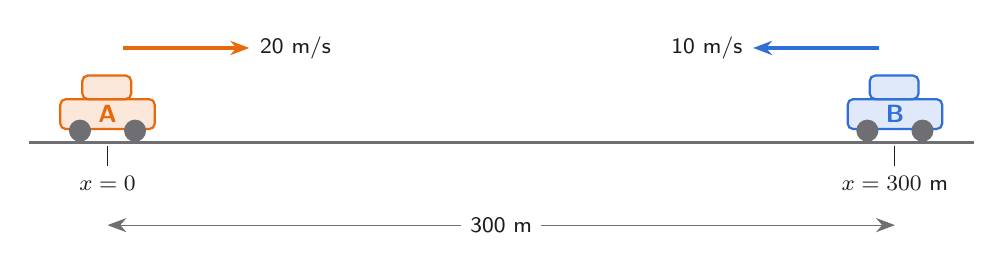
\begin{tikzpicture}[font=\footnotesize,>={Stealth[length=2.4mm]},]

\draw[thick,gris] (-1,0) -- (11,0);
\draw[thick,nar,fill=nar!15,rounded corners=2pt] (-0.6,0.17) rectangle (0.6,0.55);
\draw[thick,nar,fill=nar!15,rounded corners=2pt] (-0.32,0.55) rectangle (0.3,0.85);
\fill[gris] (-0.35,0.15) circle (0.14) (0.35,0.15) circle (0.14);\draw[thick,azul,fill=azul!15,rounded corners=2pt] (9.4,0.17) rectangle (10.6,0.55);
\draw[thick,azul,fill=azul!15,rounded corners=2pt] (9.68,0.55) rectangle (10.3,0.85);
\fill[gris] (9.65,0.15) circle (0.14) (10.35,0.15) circle (0.14);
\node[font=\small\bfseries,text=nar] at (0,0.36) {A};
\node[font=\small\bfseries,text=azul] at (10,0.36) {B};
\draw[->,very thick,nar] (0.2,1.2) -- (1.8,1.2) node[right,text=tinta] {20 m/s};
\draw[->,very thick,azul] (9.8,1.2) -- (8.2,1.2) node[left,text=tinta] {10 m/s};
\draw[tinta] (0,-0.05) -- (0,-0.3) node[below] {$x = 0$};
\draw[tinta] (10,-0.05) -- (10,-0.3) node[below] {$x = 300$ m};
\draw[<->,gris] (0,-1.05) -- (10,-1.05) node[midway,fill=white,text=tinta] {300 m};
\end{tikzpicture}
\end{document}
